\documentclass[]{ximera}
%handout:  for handout version with no solutions or instructor notes
%handout,instructornotes:  for instructor version with just problems and notes, no solutions
%noinstructornotes:  shows only problem and solutions

%% handout
%% space
%% newpage
%% numbers
%% nooutcomes

%I added the commands here so that I would't have to keep looking them up
%\newcommand{\RR}{\mathbb R}
%\renewcommand{\d}{\,d}
%\newcommand{\dd}[2][]{\frac{d #1}{d #2}}
%\renewcommand{\l}{\ell}
%\newcommand{\ddx}{\frac{d}{dx}}
%\everymath{\displaystyle}
%\newcommand{\dfn}{\textbf}
%\newcommand{\eval}[1]{\bigg[ #1 \bigg]}

%\begin{image}
%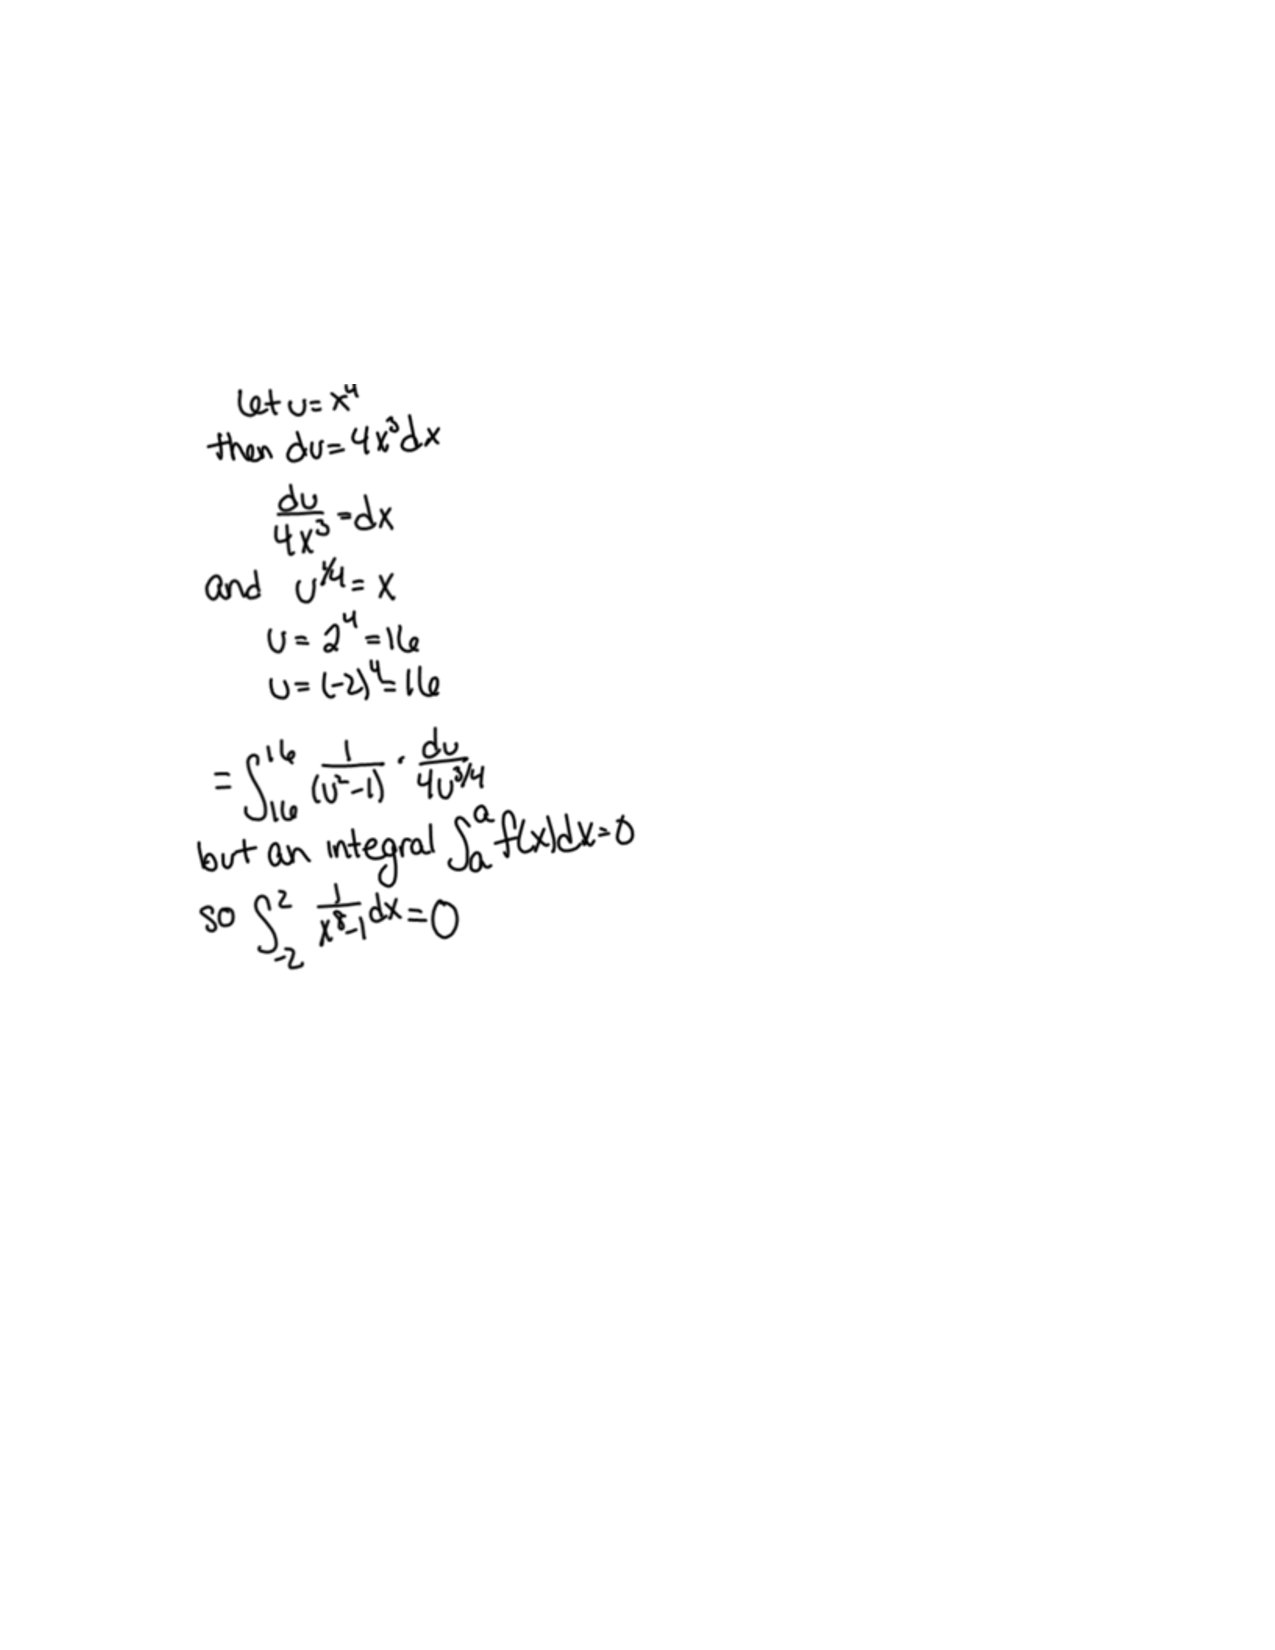
\includegraphics[trim= 170 420 250 180]{Figure1.pdf}
%\end{image}

%add a ``.'' below when used in a specific directory.
\newcommand{\RR}{\mathbb R}
\renewcommand{\d}{\,d}
\newcommand{\dd}[2][]{\frac{d #1}{d #2}}
\renewcommand{\l}{\ell}
\newcommand{\ddx}{\frac{d}{dx}}
\newcommand{\dfn}{\textbf}
\newcommand{\eval}[1]{\bigg[ #1 \bigg]}

\usepackage{multicol}

\renewenvironment{freeResponse}{
\ifhandout\setbox0\vbox\bgroup\else
\begin{trivlist}\item[\hskip \labelsep\bfseries Solution:\hspace{2ex}]
\fi}
{\ifhandout\egroup\else
\end{trivlist}
\fi} %% we can turn off input when making a master document

\title{Calculus in polar coordinates}  

\begin{document}
\begin{abstract}		\end{abstract}
\maketitle



\section{Warm up:}
True or False:  The slope of the tangent line to the curve $r = f(\theta)$ at the point $(r_0, \theta_0)$ is given by $f'(\theta_0)$.  
	\begin{freeResponse}
	{\bf False.}  The slope of the tangent line to the curve $r = f(\theta)$ at $(r_0, \theta_0)$ is given by
		\[
		\frac{\d y}{\d x} = \frac{f'(\theta_0) \sin \theta_0 + f(\theta_0) \cos \theta_0}{f'(\theta_0) \cos \theta_0 - f(\theta_0) \sin \theta_0 } \neq f'(\theta_0).
		\]
	\end{freeResponse}
	
\begin{instructorNotes}

\end{instructorNotes}







\section{Group work:}



%problem 1
\begin{problem}
Find the equation of the tangent line to $r = 2 - \sin \theta$ at $\theta = \frac{\pi}{3}$.  
Also, determine for what values of $\theta$ the tangent lines to the curve are vertical or horizontal.
	\begin{freeResponse}
	
	\end{freeResponse}
	
\end{problem}

\begin{instructorNotes}

\end{instructorNotes}







%problem 2
\begin{problem}
Graph each region and then set up an integral for the area of the region:
	\begin{enumerate}
	\item  Outside the small loop and inside the large loop of $r = 3 - 6 \sin \theta$.
	\item  Inside both of the curves $r = 4 \cos \theta$ and $r = 1 - \cos \theta$.
	\end{enumerate} 
	
	%\begin{image}
	%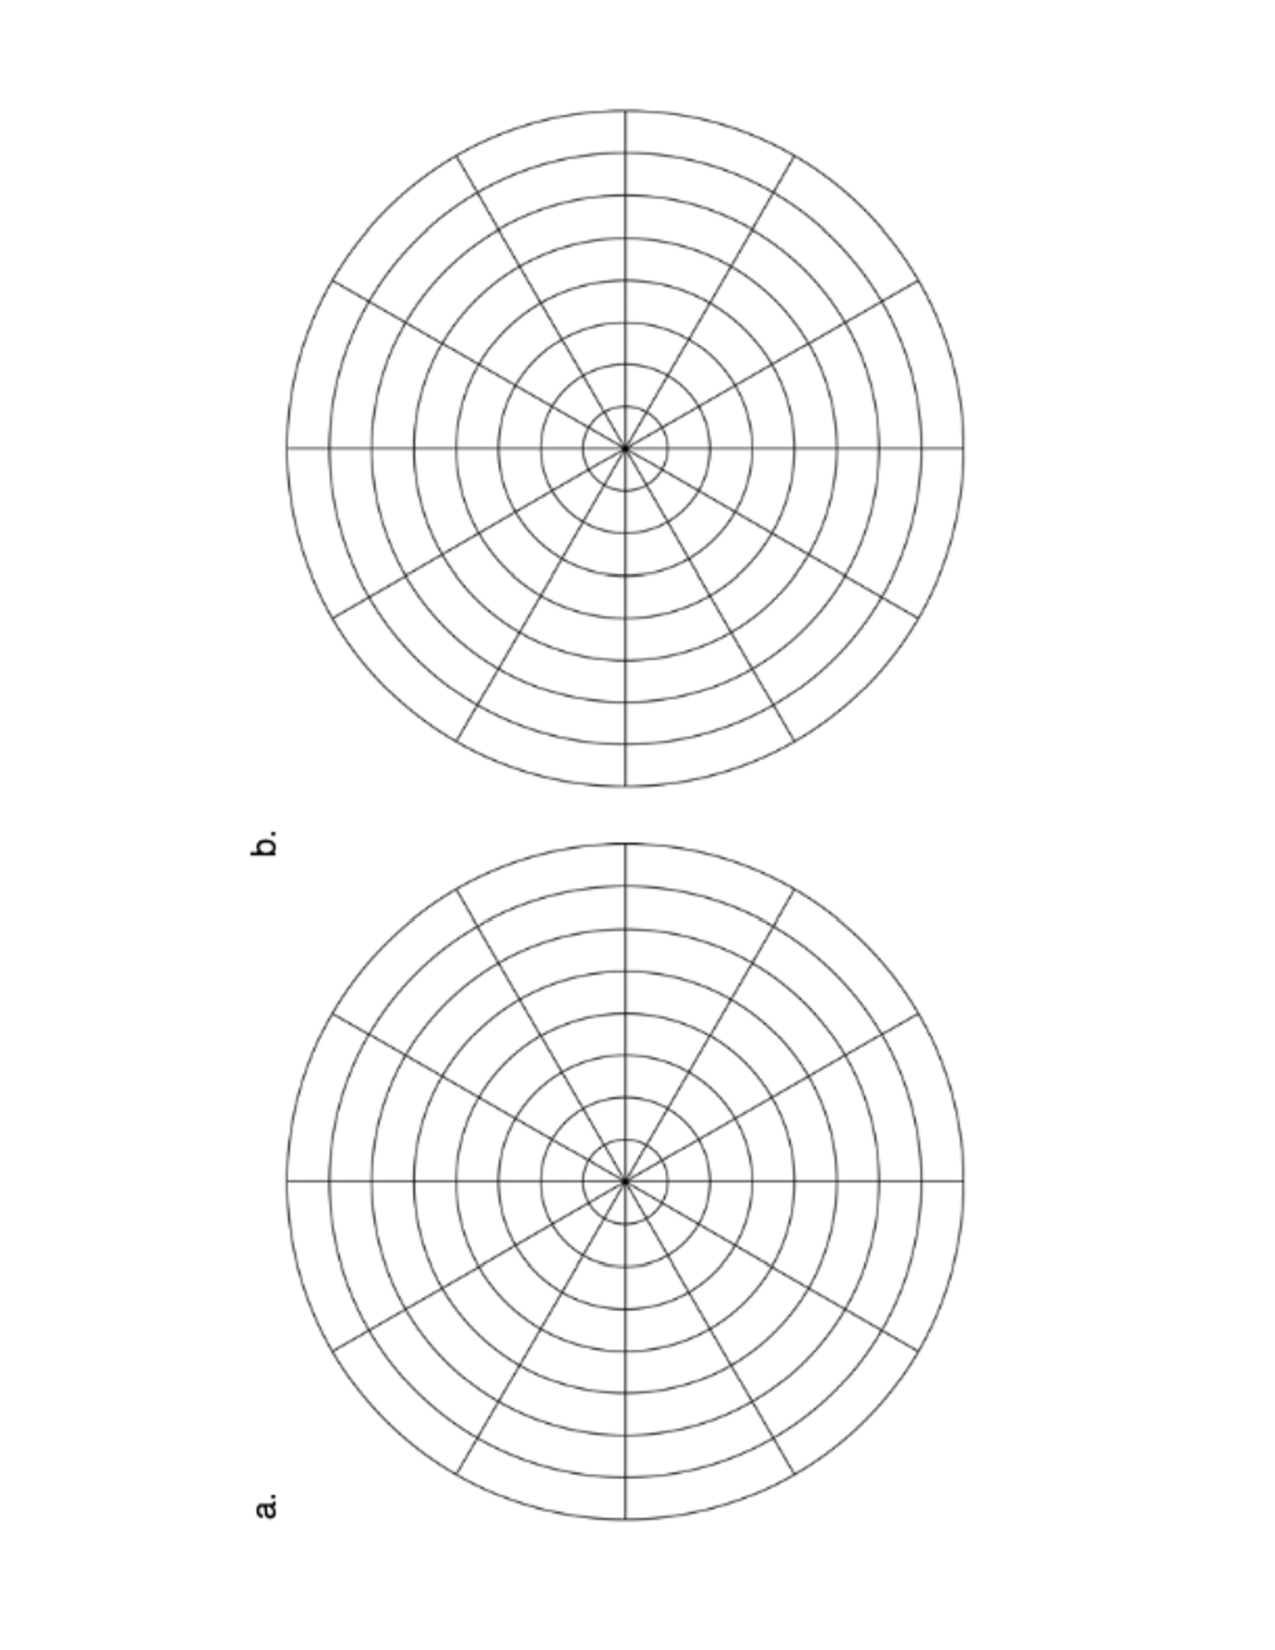
\includegraphics[trim= 170 420 250 180]{Figure11-3-1.pdf}
	%\end{image}
	
	\begin{freeResponse}
	\begin{enumerate}
	\item  
	
	\item  
	
	\end{enumerate}
	\end{freeResponse}
		
\end{problem}

\begin{instructorNotes}

\end{instructorNotes}







\begin{comment}
%problem 3
\begin{problem}

	\begin{freeResponse}
	
	\end{freeResponse}

\end{problem}

\begin{instructorNotes}

\end{instructorNotes}
\end{comment}
















	
	
	
	
	
	
	
	
	

	










								
				
				
	














\end{document} 


















